\chapter{Metodologia}

\section{Arquitetura}

\begin{figure}[htbp]
    \centering
    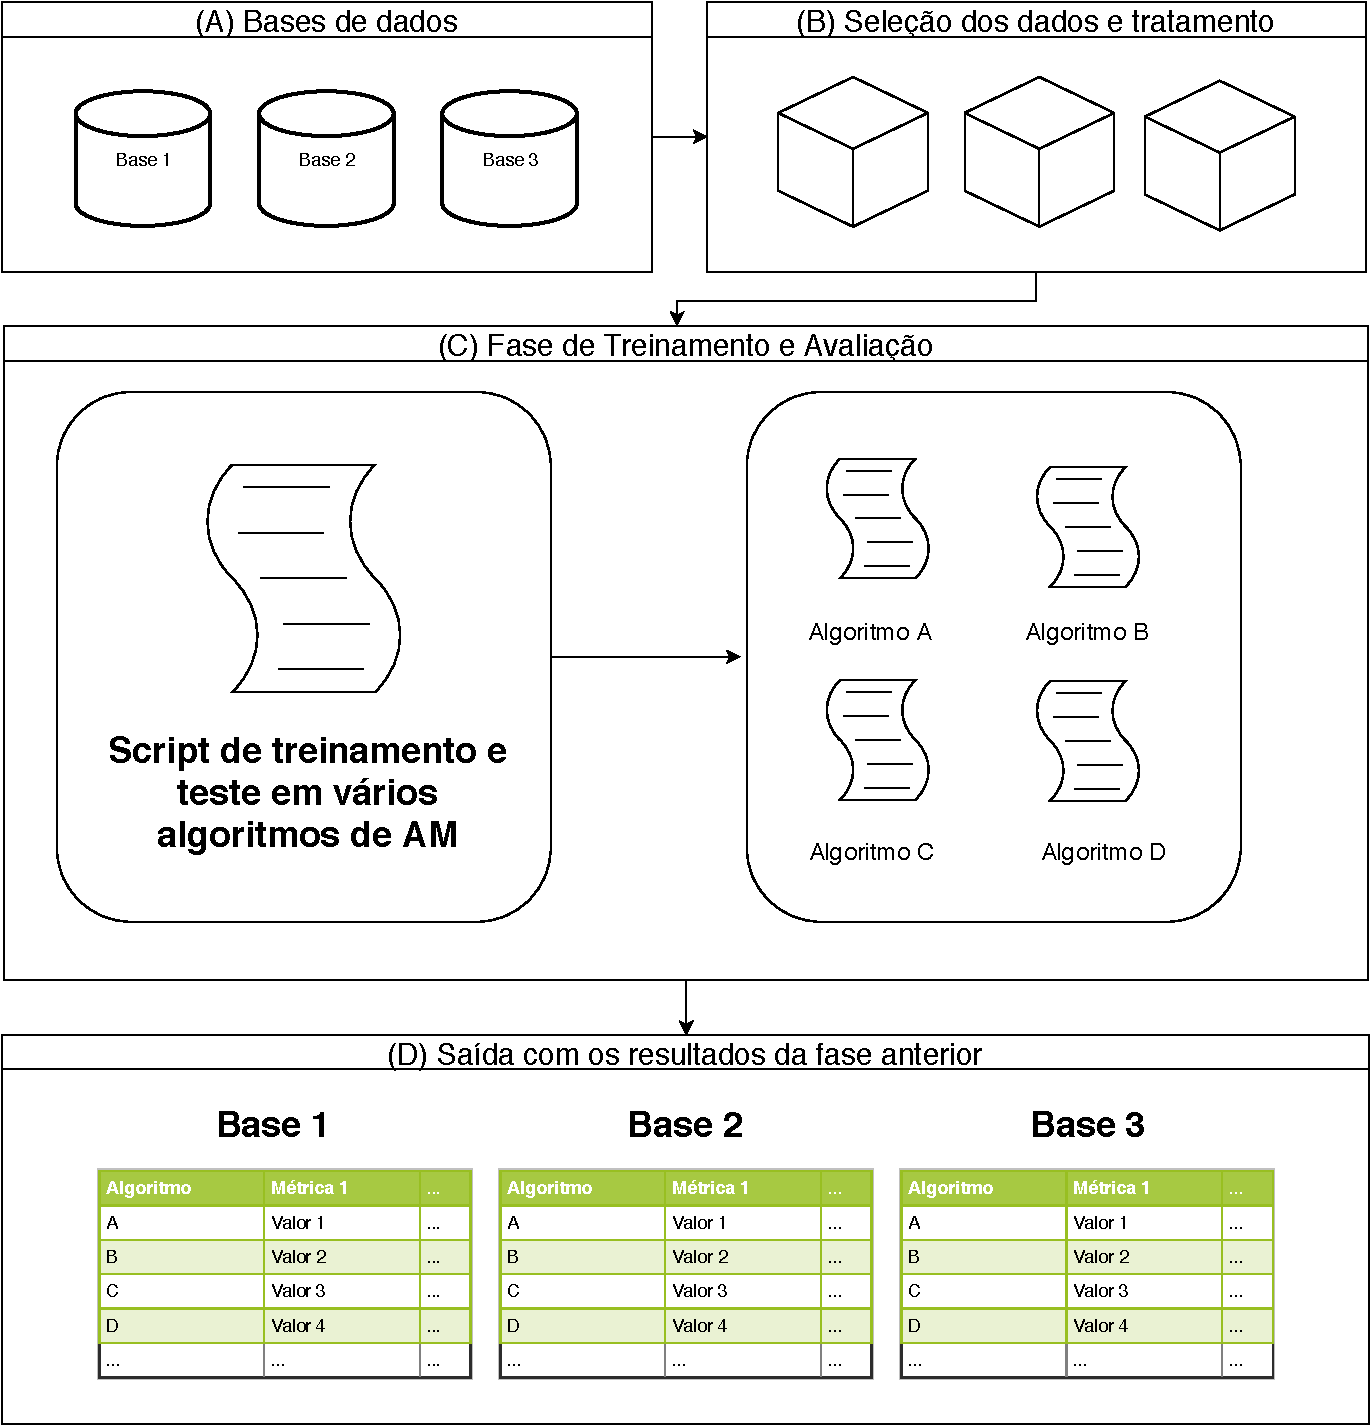
\includegraphics[width=1\textwidth]{desenvolvimento/Arquitetura.pdf}
    \caption{\label{fig:arquitetura}Arquitetura do projeto.}
    \legend{Fonte: Autor.}
\end{figure}

(isso aqui é só exemplo já que provavelmente devem haver mudanças na arquitetura)
Na Figura \ref{fig:arquitetura} as Bases de Dados (A), apresentadas na Seção \ref{basesdedados}, passam por uma fase de Seleção e Tratamento (B) para escolher, limpar e para a Fase de Treinamento e Avaliação (C)...

\section{Bases de Dados} \label{basesdedados}

Colocando links para acessar dps

HMC Software and Datasets (2008) https://dtai.cs.kuleuven.be/clus/hmcdatasets/ -- Funcat e Gene Ontology -- https://dtai.cs.kuleuven.be/clus/hmc-ens/

Catálogo Funcat -- https://web.archive.org/web/20081016031835/http://mips.gsf.de/projects/funcat/funcat20to21map -- https://www.researchgate.net/figure/Main-functional-categories-of-the-FunCat\_tbl1\_8230924

A Gene Ontology Tutorial in Python - https://www.nature.com/articles/s41598-018-28948-z -- https://pypi.org/project/goatools/

http://kt.ijs.si/DragiKocev/PhD/resources/lib/exe/fetch.php?media=clare2003.pdf

\section{Tecnologias Utilizadas}

\section{Algoritmos e Métricas de Avaliação}

\section{Configuração dos Experimentos}

